\section{Ingestion module for the PRIP file}

This section describes the ingestion module of the \acrshort{prip} reports, which contain information about the archiving of the different PDIs processed and sent by the \acrshort{pdgs}
to the \acrshort{prip}.

The associated ingestion processors are:

\begin{itemize}

\item \textbf{s2boa.ingestions.ingestion\_prip.ingestion\_prip} 

\end{itemize}

This module use the following \acrshort{dim} signatures:

\begin{itemize}

\item \textbf{PRIP\_ARCHIVING}: archiving information of the different PDIs into the \acrshort{prip}. 
    
\end{itemize}

The table \ref{tb:description_explicit_reference_ingestion_prip} shows the description of the explicit references inserted by the ingestion.

\begin{longtable}{|M{0.3\linewidth}|M{0.55\linewidth}|}
\hline \textbf{Reference} & \textbf{Description} \\ \hline
\textbf{DS PRODUCT\_ID} & Identifier of the archived DS generated by the \acrshort{pdgs} \\ \hline
\textbf{GR PRODUCT\_ID} & Identifier of the archived GR generated by the \acrshort{pdgs} \\ \hline
\textbf{TL PRODUCT\_ID} & Identifier of the archived TL generated by the \acrshort{pdgs} \\ \hline
\textbf{TC PRODUCT\_ID} & Identifier of the archived TC generated by the \acrshort{pdgs} \\ \hline
\textbf{HKTM PRODUCT\_ID} & Identifier of the archived HKTM files generated by the \acrshort{pdgs} \\ \hline
\textbf{AUX PRODUCT\_ID} & Identifier of the archived AUXILIARY files \\ \hline
\textbf{GIP PRODUCT\_ID} & Identifier of the archived GIP files \\ \hline
\caption{Table describing the explicit reference associated to the ingestion}
\label{tb:description_explicit_reference_ingestion_prip}
\end{longtable}

The figure \ref{fg:structure_ingestion_prip_annotations} shows a simplified diagram of the structure of annotations and explicit references 
inserted (associated structure of values not included for simplicity).

\begin{figure}[H]
  \begin{center}
	\centering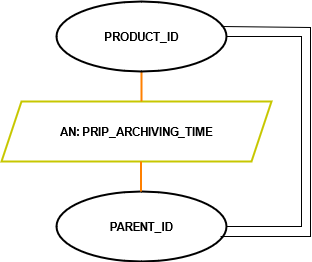
\includegraphics[scale=0.7]{../fig/structure_ingestion_prip.png}
	\caption{Structure of annotations and explicit references inserted by the ingestion module for the \acrshort{prip} file}
	\label{fg:structure_ingestion_prip_annotations}
  \end{center}
\end{figure}

Where PRODUCT\_ID includes all the different PDIs that are archived into the \acrshort{prip} (DSs, GRs, TLs, TCS, HKTM, AUX, GIP, ...) and 
the PARENT\_ID makes reference to the DSs to indicate the parent relation with the GRs, TLs and TCs (this does not apply to HKTM, AUX and GIP files). \\


The table \ref{tb:description_annotations_ingestion_prip} shows the description of the annotations inserted by the ingestion.

\begin{longtable}{|M{0.2\linewidth}|M{0.15\linewidth}|M{0.15\linewidth}|M{0.10\linewidth}|M{0.25\linewidth}|}
\hline \textbf{Annotation name} & \textbf{Annotation system} & \textbf{DIM signature} & \textbf{Insertion mode} & \textbf{Description} \\ \hline
\textbf{\acrshort{prip}\_ARCHIVING\_TIME} & None & PRIP\_ARCHIVING & INSERT\_and\_ERASE\_with\_PRIORITY & Annotation representing the \textbf{archiving details of the generated PDIs into the \acrshort{prip}} \\ \hline
\caption{Table describing the annotations associated to the ingestion}
\label{tb:description_annotations_ingestion_prip}
\end{longtable}


